\documentclass[11pt]{article}
\usepackage[a4paper,margin=1in]{geometry}
\usepackage{amsmath,amssymb,amsthm,mathtools}
\usepackage{booktabs}
\usepackage{graphicx}
\usepackage{hyperref}
\usepackage[nameinlink,capitalise]{cleveref}
\usepackage[numbers,sort&compress]{natbib}

\newtheorem{theorem}{Theorem}[section]
\newtheorem{proposition}[theorem]{Proposition}
\newtheorem{corollary}[theorem]{Corollary}
\theoremstyle{remark}
\newtheorem{remark}[theorem]{Remark}
\newcommand{\norm}[1]{\left\lVert#1\right\rVert}

\title{Rayleigh Injection Recursions for Dynamic Packet Energy\\
\large A Gap-Free Rank-Staircase Bootstrap}
\author{Liang Wang}
\date{July 2026}

\begin{document}
\maketitle

\begin{abstract}
RH-86 introduced a trace-normalized late-memory Gramian whose clock-rank
packet captures terminal postblock energy even when principal-angle
perturbation bounds are unusable.  This paper derives the scalar recursion
needed to turn that construction into an all-level proof target.

Let $\widehat G_j=X_j^*X_j/\norm{X_j}_2^2$,
$G_j=\widehat G_j+\eta G_{j-1}$, and let $E_{j,r}$ be the optimal rank-$r$
tail energy of $G_j$.  For a nondecreasing rank staircase $r_j$ and the
previous optimal packet $P_{j-1}$, the rank-staircase injection recursion is
\[
 E_{j,r_j}\le
 \underbrace{\operatorname{tr}((I-P_{j-1})\widehat G_j)}_{\iota_j}
 +\eta E_{j-1,r_{j-1}}.
\]
Iteration gives a scalar convolution of the one-step Rayleigh injections
$\iota_j$.  The current snapshot tail is at most $\sqrt{E_{j,r_j}}$, so a
uniform late-time injection estimate replaces both singular-vector matching
and spectral-gap control.

For $\eta=1/512$ and the five archived directional models, 192-bit Arb
evaluation certifies the last injection relative norm below
$4.95\times10^{-4}$ and captured snapshot energy above $0.99999975$.  The
last injection energy is at most $17.6\%$ of the preceding injection, and
every computed recursion inequality is green.  A packet available one update
earlier predicts the terminal state with relative residual below
$1.19\times10^{-3}$; at the four finer scales the bound is below
$4.1\times10^{-6}$.

This is a rigorous reduction plus finite-scale evidence, not an all-level
injection law.  Stage A, Hilbert--Polya, and the Riemann Hypothesis remain
open.
\end{abstract}

\noindent\textbf{Keywords:} Rayleigh injection; dynamic packet; Ky Fan tail;
rank staircase; scalar recursion; interval arithmetic.

\medskip
\noindent\textbf{MSC 2020:} 47A75; 47B10; 15A18; 65G20.

\section{The scalar quantity behind packet drift}

RH-85 proved that a prefix packet can be propagated to the terminal state
\citep{WangSnapshot2026}.  RH-86 replaced a single packet snapshot by the
online normalized memory
\citep{WangMemory2026}
\[
 G_j=\widehat G_j+\eta G_{j-1},\qquad
 \widehat G_j=\frac{X_j^*X_j}{\norm{X_j}_2^2}.
\]
Its leading eigenspace minimizes the weighted relative residual, but directly
tracking that eigenspace is ill-conditioned.  The missing invariant is the
energy injected by the new snapshot outside the old packet.

For a positive trace-class operator $G$, write
\[
 E_r(G)=\operatorname{tr}G-\sum_{k=1}^r\lambda_k(G).
\]
Let $P_{j,r}$ denote any leading rank-$r$ projection of $G_j$.

\section{Rank-staircase injection recursion}

\begin{theorem}[Rank-staircase injection recursion]
\label{thm:recursion}
Let $r_j$ be nondecreasing and put $P_{j-1}=P_{j-1,r_{j-1}}$.  Then
\begin{equation}
 \boxed{
 E_{r_j}(G_j)\le \iota_j+\eta E_{r_{j-1}}(G_{j-1}),
 \qquad
 \iota_j=\operatorname{tr}((I-P_{j-1})\widehat G_j).}
 \label{eq:recursion}
\end{equation}
Moreover,
\begin{equation}
 \frac{\norm{X_j(I-P_{j,r_j})}_2^2}{\norm{X_j}_2^2}
 \le E_{r_j}(G_j).
 \label{eq:current}
\end{equation}
\end{theorem}

\begin{proof}
Because $r_{j-1}\le r_j$, the old projection is an admissible rank-at-most
$r_j$ candidate in Ky Fan's variational principle.  Therefore
\begin{align*}
 E_{r_j}(G_j)
 &\le\operatorname{tr}((I-P_{j-1})G_j)\\
 &=\operatorname{tr}((I-P_{j-1})\widehat G_j)
 +\eta\operatorname{tr}((I-P_{j-1})G_{j-1})\\
 &=\iota_j+\eta E_{r_{j-1}}(G_{j-1}).
\end{align*}
The current normalized snapshot is a nonnegative weight-one summand in the
optimal memory residual, giving \eqref{eq:current}.
\end{proof}

The theorem is gap free.  It also allows a rank jump: retaining the old
rank-$r_{j-1}$ packet is already admissible at rank $r_j$, and any extra
directions can only improve the bound.

\begin{corollary}[Scalar convolution corollary]
\label{cor:convolution}
For $b<j$,
\begin{equation}
 E_{r_j}(G_j)
 \le \eta^{j-b}E_{r_b}(G_b)
 +\sum_{t=b+1}^j\eta^{j-t}\iota_t.
 \label{eq:convolution}
\end{equation}
If $\iota_t\le\bar\iota$ after $b$, then the second term is at most
$\bar\iota/(1-\eta)$.  If the injections decay geometrically, the right side
is the convolution of two geometric sequences.
\end{corollary}

\begin{proof}
Iterate \eqref{eq:recursion}.  The two stated bounds follow by summing the
resulting geometric series.
\end{proof}

This formula makes the analytic wall precise: prove a late-time scalar bound
for $\iota_t$ at the half-logarithmic rank.  No individual singular value,
principal angle, or coordinate packet must be identified.

\section{Five-scale injection audit}

The audit uses $r=\lceil H_\sigma\rceil+2$, $\eta=1/512$, and packet time
$j=\lceil2M/3\rceil$.  The full memory recursion is computed in binary64.
The final injection uses the packet at $j-1$ and the exact lifted snapshot at
$j$; its residual is evaluated in 192-bit Arb arithmetic.  The same lagged
packet is propagated to $M$ and evaluated directly.

\begin{table}[ht]
\centering
\small
\begin{tabular}{rrrrr}
\toprule
$\sigma$ & worst $\sqrt{\iota_j}$ & max $\iota_j/\iota_{j-1}$ & lagged terminal & max utilization\\
\midrule
0.16 & $4.95\times10^{-4}$ & 0.0984 & $1.19\times10^{-3}$ & 0.0071\\
0.08 & $2.54\times10^{-6}$ & 0.0719 & $4.02\times10^{-6}$ & 0.0344\\
0.04 & $2.68\times10^{-7}$ & 0.0254 & $1.43\times10^{-6}$ & 0.1281\\
0.02 & $5.32\times10^{-7}$ & 0.1362 & $6.55\times10^{-7}$ & 0.5276\\
0.01 & $2.68\times10^{-7}$ & 0.1757 & $1.75\times10^{-7}$ & 0.3284\\
\bottomrule
\end{tabular}
\caption{Worst directional result at each scale.  Utilization is
$E_j/(\iota_j+\eta E_{j-1})$ for the final update.}
\label{tab:audit}
\end{table}

The coarse right channel is predictive but not yet in the $10^{-5}$ regime
one update early.  The four finer levels are substantially stronger.  At all
scales the final injection is decreasing relative to the immediately
preceding injection, and the scalar recurrence retains positive slack.

\begin{figure}[ht]
\centering
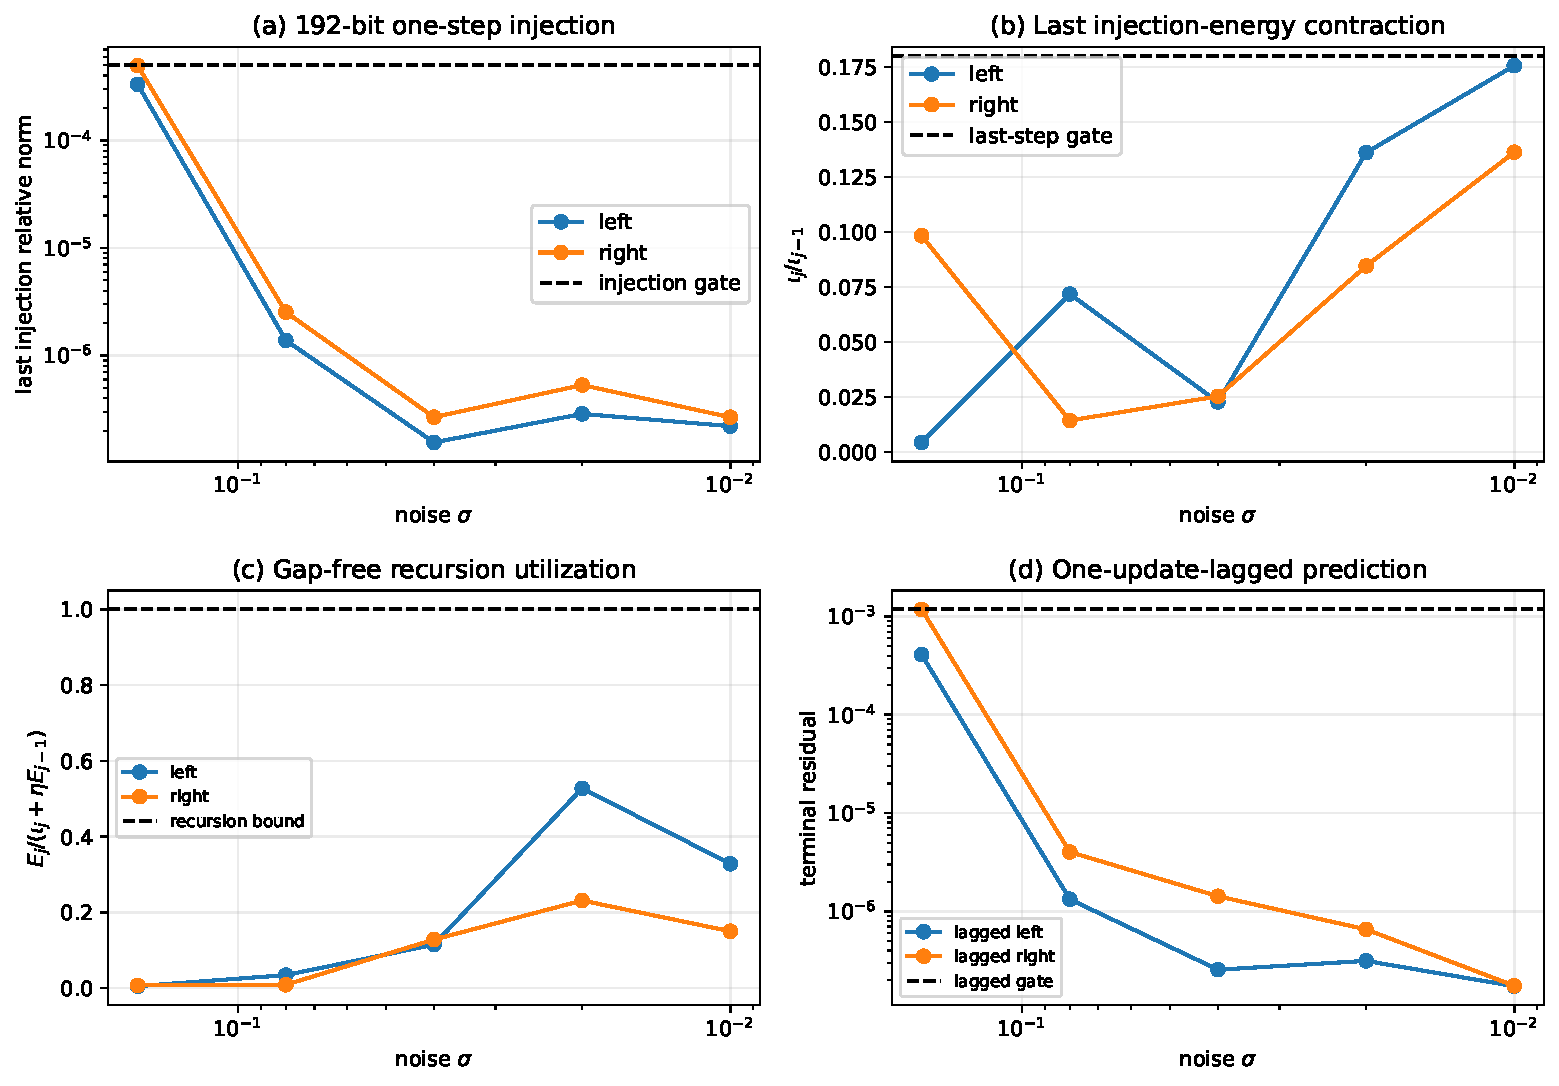
\includegraphics[width=\textwidth]{figures/rayleigh_injection_recursion.pdf}
\caption{Validated final injection, last-step contraction, recursion
utilization, and one-update-lagged terminal prediction.}
\label{fig:audit}
\end{figure}

\section{Boundary and next theorem}

RH-87 converts the dynamic packet problem into a one-dimensional sequence.
The next theorem should estimate $\iota_j$ from one-step normalized Gram data,
ideally by decomposing it into transported old-packet leakage and a finite-rank
source-injection term.  A useful all-level statement would give a burn-in
$b_\sigma=O(\log^2(1/\sigma))$ and a geometric or polylogarithmic bound on
$\iota_j$ thereafter.

The exact recursion does not prove that bound.  The finite audit does not
close the all-level injection law, Stage A1 or Stage A4, a relative fixed-disk
determinant, a self-adjoint Hilbert--Polya operator, a zeta-zero identity, or
the Riemann Hypothesis.

\bibliographystyle{plainnat}
\bibliography{references}

\end{document}
